Games and other virtual applications are based on mathematical models and often times need to be calculated in real-time on a computer system. The most common operations and algorithms for capturing and reconstructing 3-D models involve vectors and matrices, which are also the main concepts the MATLAB programming language is built on. Other commonly used branches of mathematics in computer vision are trigonometry, algebra, statistics and calculus (\cite[p.165]{Gregory.2014}).

The following sections shall introduce the mathematical backgrounds of some of the most important algorithms in computer vision. For this, the basic 2-D and 3-D primitives in combination with the 3-D to 2-D projection need to be discussed first. Mathematical problems in multiple view geometry can often be broken down into 2-D space problems. Readers who have already studied computer graphics can skip the basic chapters. The explanations shall only serve as an overview and summary of the topics (\cite[p.29]{Szeliski.2011} and (\cite[p.165 et seq.]{Gregory.2014}).

%%%%%%%%%%%%%%%%%%%%%%%%%%%%%%%%%%%%%%%%%%%%%%%%%%
\section{Projective and Single-View Geometry}
%%%%%%%%%%%%%%%%%%%%%%%%%%%%%%%%%%%%%%%%%%%%%%%%%%
Three-dimensional shapes can be described with geometrical primitives, such as points, lines and planes. A virtual world is created out of such 3-D objects, which all have a position, orientation and scale. Typically, geometry needs to start with a \textit{point} (\cite[p.29 et seqq.]{Szeliski.2011} and \cite[p.166 et seqq.]{Gregory.2014}).

\subsection{2-D and 3-D points}\label{ssec:Points}
\index{Points}
A 2-D point\index{Points!2-D points} can represent a pixel coordinate in an image and can be described as an ordered pair of real numbers 
\begin{equation}
\mathbf{x} = (x,y)\in \mathbb{R}^2
\end{equation}

or alternatively, 
\begin{equation} 
\mathbf{x}=
  \begin{bmatrix}
   x \\
   y
  \end{bmatrix}
\end{equation}

Points have \textit{equivalence classes}\index{Points!Equivalence classes}, which are represented by adding an extra coordinate, creating a coordinate triple. This means that $x=(x,y,1)$, $x=(2x,2y,2)$ and $x=(kx,ky,k)$, for any $k\neq0$, represent the same point, they only differ by a multiple. By dividing through $k$ the original coordinates are retrieved. These coordinate triples are called \textit{homogeneous coordinates}\index{Homogeneous coordinates}. The equation $x=(x,y,0)$ represents a \textit{point at infinity}\index{Points!Point at infinity}, since the coordinate points can not be divided by $0$. Those points form a line in the two-dimensional projective space, which is called the \textit{line at infinity}\index{Line at infinity} (\cite[p.30]{Szeliski.2011} and \cite[p.2]{Hartley.2011}).

The same principles apply for points in three-dimensional coordinate systems. Thus, a 3-D point \index{Points!3-D points} can be represented using inhomogeneous coordinates:
\begin{equation}
\mathbf{x} = (x,y,z)\in \mathbb{R}^3
\end{equation}  

or alternatively using homogeneous coordinates by adding another coordinate:
\begin{equation}
\mathbf{x} = (x,y,z,w)\in \mathbb{P}^3
\end{equation}  

Note that the \textit{points at infinity} in 3-D space form the \textit{plane at infinity}\index{Plane at infinity} (\cite[p.31]{Szeliski.2011} and \cite[p.2]{Hartley.2011}).

\subsection{Coordinate Systems}
\paragraph{Types of coordinate systems.}
As stated above, a point is represented with its coordinates in a $n$-dimensional space, whereas in computer vision $n$ usually has the value $2$ or $3$. Hence, coordinate systems\index{Coordinate systems} play an important role in computer vision tools. While the \textit{Cartesian coordinate system} is the most commonly used coordinate system in the field, it is certainly not the only one. The following list will introduce three important coordinate systems, which use different concepts: (\cite[p.166 et seq.]{Gregory.2014}.  
\begin{enumerate}[i]
\item \textit{Cartesian coordinate systems}\index{Coordinate systems!Cartesian coordinate system}: Two or three fixed perpendicular axis which form the 2-D or 3-D space. The points are represented by $(P_x,P_y)$ or $(P_x,P_y,P_z)$ and an illustration can be seen in \autoref{fig:CoordinateSys}.  
\item \textit{Cylindrical coordinate systems}\index{Coordinate systems!Cylindrical coordinate system}: A system with a vertical axis $h$, a radial axis $r$ and the yaw angle $\Theta$. The points are represented by $(P_h,P_r,P_\Theta)$
\item \textit{Spherical coordinate systems}\index{Coordinate systems!Spherical coordinate system}: A system specified by the radial distance $r$ of a point from the origin, the yaw angle $\Theta$ and a pitch angle $\phi$. Thus, a point is represented by $(P_r,P_\phi,P_\Theta)$.
\end{enumerate}

This thesis is concentrating on points represented in the Cartesian coordinate system, since it is the most used system in computer graphics and computer vision environments.

\paragraph{Left-handed vs. right-handed orientation.}
\index{Coordinate systems!Left-handed}\index{Coordinate systems!Right-handed}
Three-dimensional Cartesian coordinate systems can be arranged in two different directions: right-handed and left-handed. They differ only in the orientation of one of the three axis, for example the $z$-axis points to the front in a right-handed, and to the rear in a left-handed coordinate system (as illustrated in \autoref{fig:CoordinateSys}). Often the $y$-axis points downwards, defining a left-handed coordinate system. The resulting point representations in both systems are not much different from each other: by negating the $y$-coordinate of the points the coordinate system becomes right-handed. Also it is important to note that the actual position of the point in space does not change, it is only the interpretation of it which is defined by this orientation. It is up to the programmer to chose a system and it is important to be consistent throughout one environment (\cite[p.164 et seq.]{Hartley.2011} and \cite[p.167 et seq.]{Gregory.2014}). 

\begin{figure}[htbp]
		\centering
		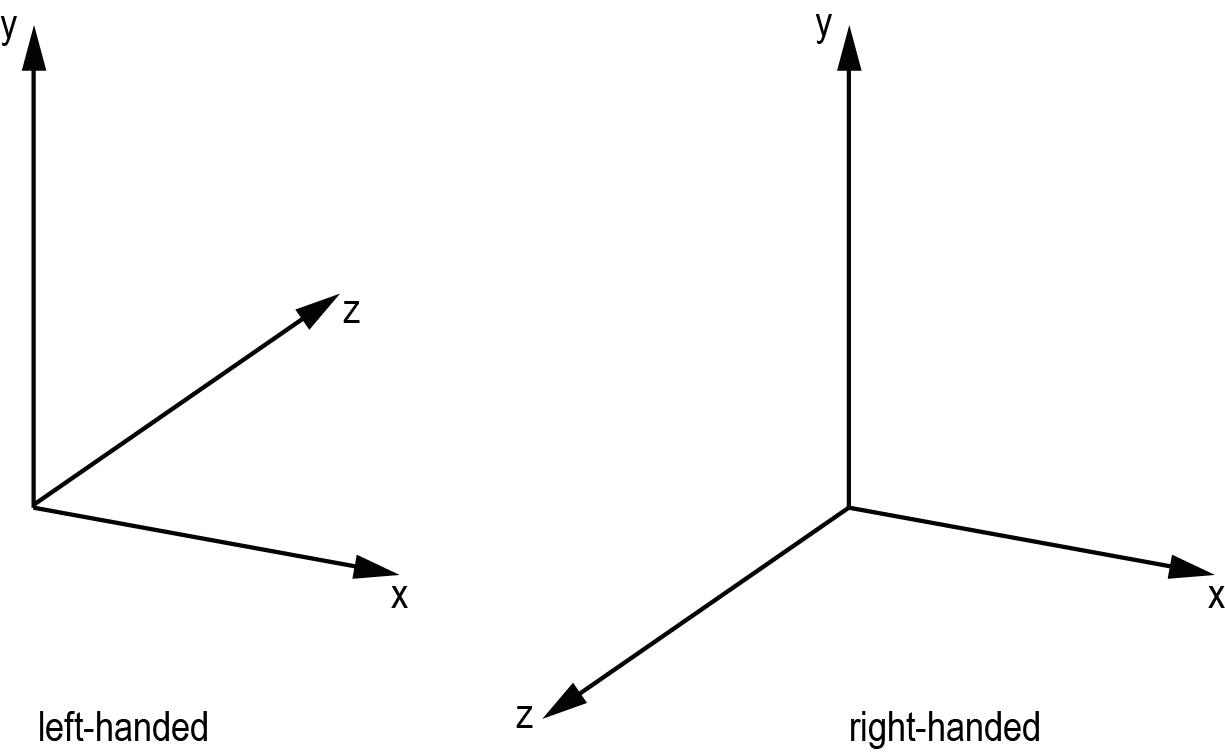
\includegraphics[width=0.8\textwidth]{figures/CoordinateSystems}
		\caption[Left- and right-handed Cartesian coordinate systems]{Left- and right-handed Cartesian coordinate systems (\textit{source: own illustration based on} \cite[p.167]{Gregory.2014}).}
		\label{fig:CoordinateSys}
\end{figure}

\subsection{3-D to 2-D Projections}\label{ssec:projection}
To display a model of the 3-D world on a computer screen one has to map the 3-D objects to a 2-D representation. In this process the 3-D structure gets projected on a two-dimensional image, losing one dimension. Thus, there is a minimum of two coordinate systems involved: the world-space\index{Coordinate systems!World-space} and the 2-D image coordinates. Their relationship to each other can be modeled with the help of a \textit{central projection}\index{Projection!Central projection}: a ray from a point $X_i$ in real world space (\textit{world point}) passes through the fixed \textit{center of projection}\index{Projection!Center of projection} $C$ and intersects with the \textit{image plane} (as seen in \autoref{fig:Projection}). This intersection $x_i$ represents the image of the real world point $X_i$ (\cite[p.6 et seq.]{Hartley.2011}).

\begin{figure}[htbp]
		\centering
		\includegraphics[width=0.6\textwidth]{figures/Projection}
		\caption[Projection of the world points $X_i$ to the image plane through $C$]{Projection of the world points $X_i$ to the image plane through the center of projection $C$ (\textit{source: own illustration based on} \cite[p.8]{Hartley.2011}).}
		\label{fig:Projection}
\end{figure}

This model can be seen as a simple camera, in which the center of projection is the lens of the camera. The mapping from the projective spaces $\mathbb{P}^3$ to $\mathbb{P}^2$ may be represented by a $3\times4$ matrix $P$, which takes the homogeneous coordinates $(X,Y,Z,T)^T$ of a point in $\mathbb{P}^3$ and the center of projection into account. The most general imaging projection is known as the \textit{camera matrix}\index{Camera matrix} $P$. Hence, the projection of a three-dimensional world point (in its homogeneous coordinates) to a two-dimensional image point (in its homogeneous coordinates) with this simple camera concept can be expressed as (\cite[p.7]{Hartley.2011} and \cite[p.42 et seqq.]{Szeliski.2011}):

\begin{equation} 
 \begin{pmatrix}
  x \\
  y \\
  w
 \end{pmatrix} = P_{3\times4}
 \begin{pmatrix}
  X \\
  Y \\
  Z \\
  T
 \end{pmatrix}\label{eq:camMatrix}
\end{equation}

\subsection{The projective Camera}\label{ssec:projCam}
Real-world 3-D objects can be reconstructed by using one or multiple cameras to digitize them (later chapters will cover this process in more detail). As stated above, a camera is the mapping of the 3-D world space to a 2-D image. This mapping is represented with certain matrices $P$\index{Camera matrix}. Thinking of real cameras one has to take their own properties, like their focal length and aspect ratio, into account as well. These properties are called \textit{internal camera parameters} or \textit{intrinsics}\index{Intrinsic camera parameters} and are stored in a $3\times 3$ matrix $K$ (\cite[p.152 et seq.]{Hartley.2011}).

Cameras can be classified into \textit{finite cameras}\index{Finite cameras} and cameras which have their center at infinity (e.g. \textit{affine cameras}\index{Affine camera} for parallel projection\index{Projection!Parallel projection}). Each camera model has its own matrix which represents its particular camera mapping. The models important for this thesis are using the \textit{central projection} (see \autoref{eq:camMatrix}) as the basic principal (\cite[p.153]{Hartley.2011}).

\paragraph{The pinhole camera.} The pinhole camera\index{Pinhole camera} is the simplest finite camera model and shall serve as an introduction for \textit{projective geometry} and its mathematical expressions. The mapping of a pinhole camera model can be expressed by rewriting \autoref{eq:camMatrix} as:
\begin{equation} 
 \begin{pmatrix}
  X \\
  Y \\
  Z \\
  1
 \end{pmatrix}\longmapsto
 \begin{pmatrix}
  fX \\
  fY \\
  Z
 \end{pmatrix}=
 \begin{bmatrix}
  f & & & 0\\
   & f & & 0 \\
   &  & 1 & 0
 \end{bmatrix}
 \begin{pmatrix}
  X \\
  Y \\
  Z \\
  1
 \end{pmatrix}
\end{equation}
with $Z = f$ as the \textit{image plane} or \textit{focal plane} and the world-point $\mathbf{X}=(X,Y,Z)^T$. The right part of the equation consists of the multiplication between the camera matrix $P$ for the pinhole model and the world point in homogeneous coordinates. Alternately $P$ can be written as $P=diag(f,f,1)[ I | 0]$. With this the image point can be written in short as (\cite[p.153 et seq.]{Hartley.2011}):
\begin{equation}
 \mathbf{x}=P\mathbf{X}
\end{equation}

Taking into account the fact that the origin of coordinates in the image plane may not be at the \textit{principal point}\index{Principal point} $(p_x, p_y)^T$, this principle point offset must be addressed with (\cite[p.155]{Hartley.2011}):
\begin{equation} 
 \begin{pmatrix}
  X \\
  Y \\
  Z \\
  1
 \end{pmatrix}\longmapsto
 \begin{pmatrix}
  fX+Zp_x \\
  fY+Zp_y \\
  Z
 \end{pmatrix}=
 \begin{bmatrix}
  f & & p_x & 0\\
   & f & p_y & 0 \\
   &  & 1 & 0
 \end{bmatrix}
 \begin{pmatrix}
  X \\
  Y \\
  Z \\
  1
 \end{pmatrix}\label{eq:princPt}
\end{equation} 

Whereas 
\begin{equation}
 K=
 \begin{bmatrix}
  f & & p_x\\
   & f & p_y\\
   &  & 1
 \end{bmatrix}
\end{equation}
is the \textit{camera calibration matrix}. \autoref{eq:princPt} can then be written in short as 
\begin{equation}
 \mathbf{x}=K[I|0]\mathbf{X}_{cam}\label{eq:princPtShort}
\end{equation}

\paragraph{Camera rotation and translation}
Real world points are usually expressed in a different coordinate system of their own: the \textit{world coordinate system} or \textit{world frame or space}\index{Coordinate systems!World-space}. This system stands in relation to the camera coordinate system via a rotation and translation as illustrated in \autoref{fig:CoordinateSystemRT}.

\begin{figure}[htbp]
		\centering
		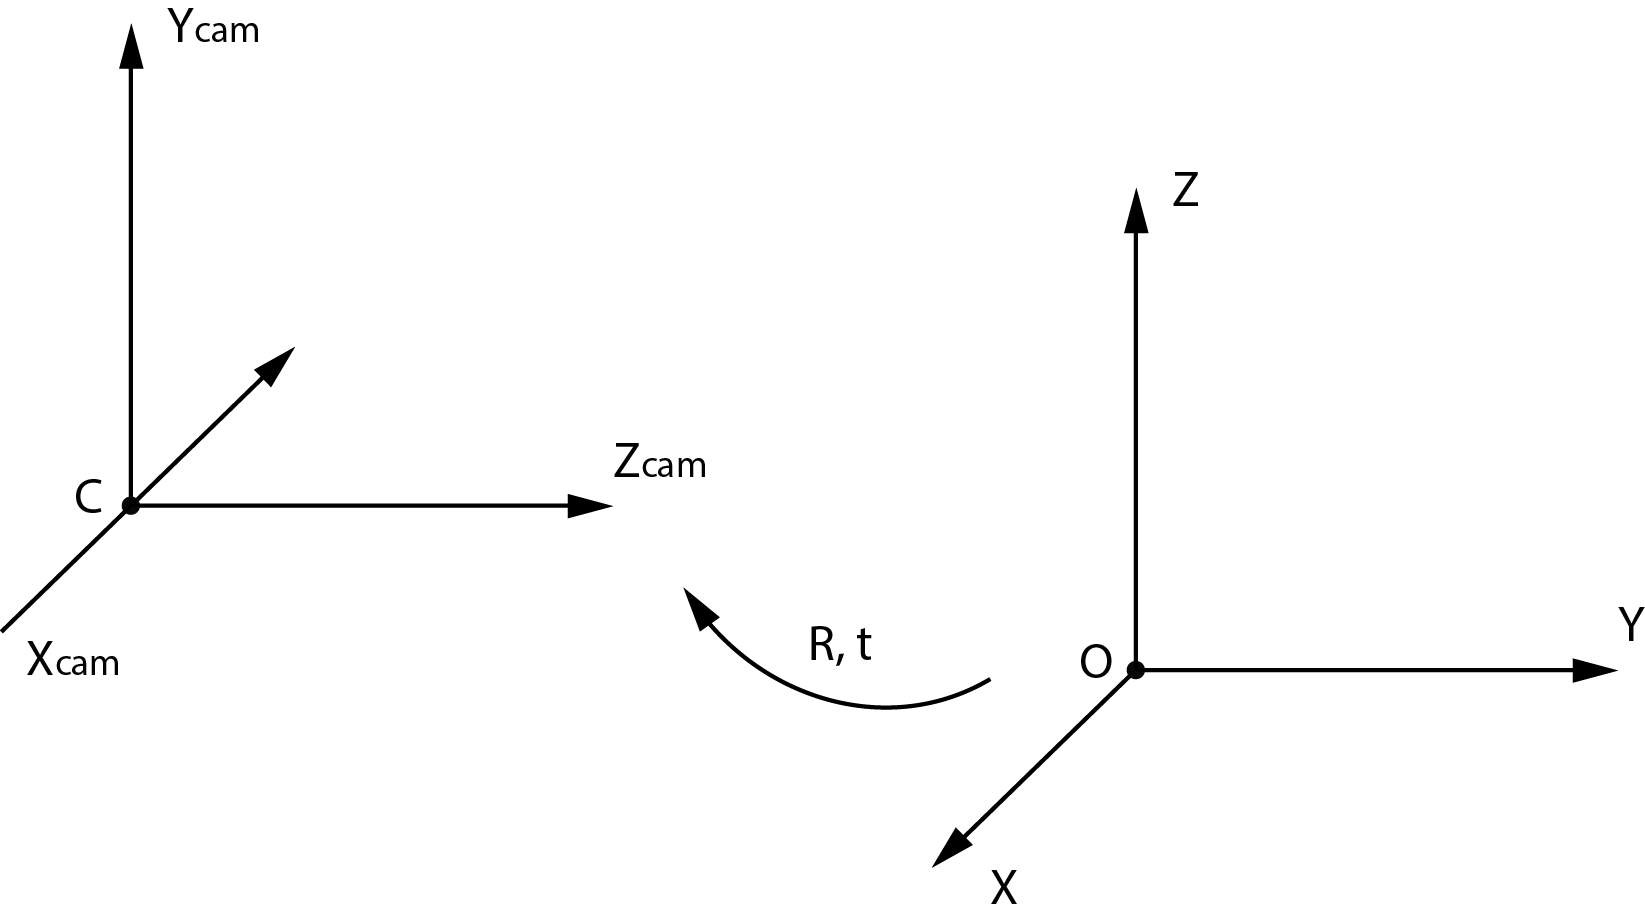
\includegraphics[width=0.8\textwidth]{figures/CoordinateSystemRT}
		\caption[Transformation between world and camera coordinate systems]{Transformation between world and camera coordinate systems (\textit{source: own illustration based on} \cite[p.156]{Hartley.2011}).}
		\label{fig:CoordinateSystemRT}
\end{figure}

The rotation $R$ is represented by a $3\times 3$ matrix. The image of a world point in the camera coordinate system is then equated with (\cite[p.155 et seq.]{Hartley.2011}):

\begin{equation}
 \mathbf{X}_{cam}=
 \begin{bmatrix}
  R & -R\tilde{C} \\
  0 & 1
 \end{bmatrix}
 \begin{pmatrix}
  X \\
  Y \\
  Z \\
  1
 \end{pmatrix}=
 \begin{bmatrix}
  R & -R\tilde{C} \\
  0 & 1
 \end{bmatrix}\mathbf{X}
\end{equation}
whereas $\tilde{C}$ represents the camera center in world coordinates.
In combination with \autoref{eq:princPtShort} this leads to the general mapping given by a pinhole camera:

\begin{equation}
 \mathbf{x}=KR[I|-\tilde{C}]\mathbf{X}\label{eq:pinholeMapping}
\end{equation}

with $\mathbf{X}$ now written in world coordinates, $K$ representing the \textit{internal camera parameters} and $R$ and $\tilde{C}$ representing the \textit{external camera parameters}\index{Extrinsic camera parameters} giving a projective camera 11 independent transformation parameters (\cite[p.156 et seq.]{Hartley.2011} and \cite[p.274]{Luhmann.2014}. 
\todo{extrinsics, intrinsics --> compare with matlab}

\note{For computer vision the Euclidean space $\mathbb{R}^n$ is problematic in many ways. Parallel lines meet \enquote{at infinity}, which is merely a model but typically all points are equal in the real world - there is no origin. Euclidean as well as affine transformations \enquote{preserve}\footnote{Points at infinity remain points at infinity even after computations.} points at infinity, making them different. For convenience, computer vision uses the projective space $\mathbb{P}^n$ to map 3-D objects to 2-D images. This is achieved by extending the Euclidean space with a line (or a plane) at infinity. Now points at infinity are not any different than other points and they are projected to other points with projective transformations. A projective camera therefore is a map from $\mathbb{P}^3$ to $\mathbb{P}^2$. However, it is still important to remember that cameras are Euclidean devices (\cite[p.1 et seqq. and 165]{Hartley.2011}).}

\todo{spell-check from here}\\
%%%%%%%%%%%%%%%%%%%%%%%%%%%%%%%%%%%%%%%%%%%%%%%%%%
\section{Epipolar and Two-View Geometry}
%%%%%%%%%%%%%%%%%%%%%%%%%%%%%%%%%%%%%%%%%%%%%%%%%%
One way to recover 3-D structure is to use the data of two (or multiple) camera views to search for corresponding points in image planes to calculate the absolute position of these points in world space. This section will cover the topic of \textit{epipolar geometry}\index{Epipolar geometry} which describes the intrinsic projective relationship between two views. Those two views can be either taken with two cameras simultaneously or with only one camera sequentially, which is geometrically equivalent. Both views have their own camera matrix $P,P'$ and their own sets of image points $\mathbf{x}=P\mathbf{X}$ and $\mathbf{x'}=P'\mathbf{X}$, whereas $\mathbf{x}$ and $\mathbf{x'}$ are called \textit{corresponding points}\index{Corresponding points} since they represent the same 3-D world point $\mathbf{X}$ just from different viewing perspectives (\cite[p.238]{Hartley.2011}).

The in this chapter discussed concepts can address the following issues (freely adapted from \cite[p.238]{Hartley.2011}):
\begin{enumerate}[i]
\item \textbf{Correspondences geometry:} Retrieving the image point $\mathbf{x'}$ with the given corresponding image point $\mathbf{x}$.
\item \textbf{Camera geometry:} Retrieving the camera matrices $P$ and $P'$ with the given set of corresponding image points. 
\item \textbf{Scene geometry:} Retrieving the position of the 3-D world point $\mathbf{X}$ with the given set of corresponding image points and the two known camera matrices $P$ and $P'$. 
\end{enumerate}

\subsection{The Structure of Epipolar Geometry}
\begin{figure}[htbp]
		\centering
		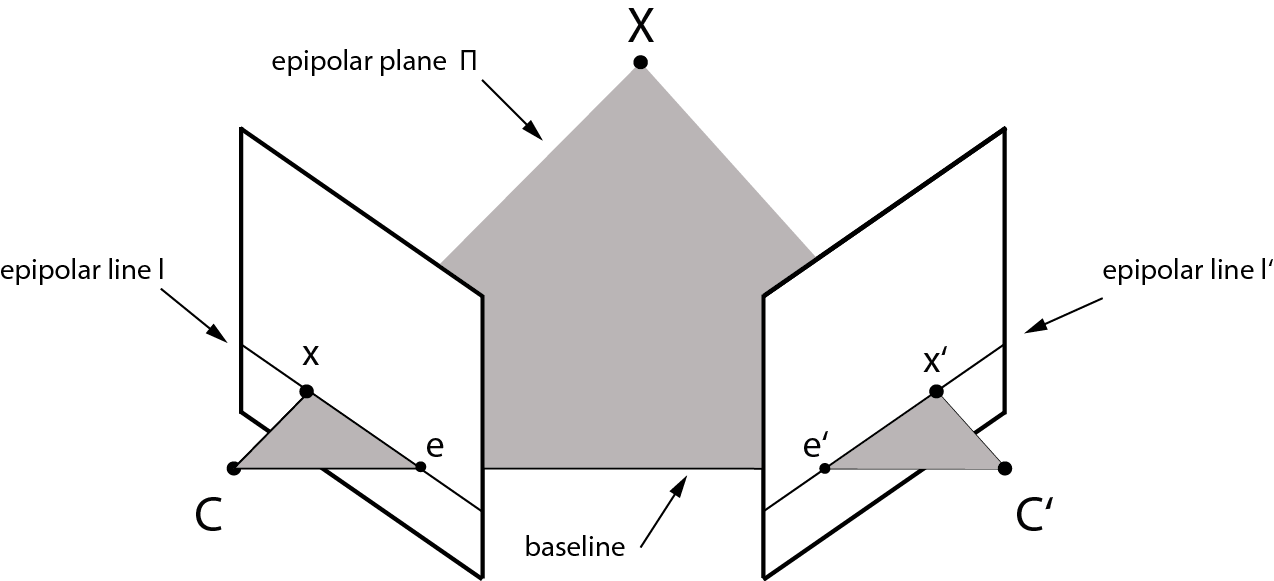
\includegraphics[width=1.0\textwidth]{figures/EpipolarGeometry}
		\caption[Involved entities of the point correspondence geometry]{Involved entities of the point correspondence geometry (\textit{source: own illustration based on} \cite[p.240]{Hartley.2011}).}
		\label{fig:Epipolar}
\end{figure}

First, the structure of the relationship between the two views shall be defined (\autoref{fig:Epipolar} illustrates the entities involved). The two \textit{camera centers} $C$ and $C'$ are connected through the \textit{baseline}\index{Baseline}, which also defines the axis of a pencil of image planes\footnote{The word \textit{pencil} means here a family of geometric objects with certain common properties, such as common lines, etc.}. A \textit{3-D world point} $X$ gets projected onto the two image planes as the points $x$ in the first camera view and as $x'$ in the second.  $X$, $x$ and $x'$ are \textit{coplanar} - they lie in the plane $\pi$. Most importantly, the rays back-projected from the two image points, intersecting in $X$ also lie in $\pi$. This means that the plane $\pi$ can be defined by the baseline and the ray from $x$. Going further, $x'$ then needs to lie on $l'$, which is the image in the second view of the back-projected ray from $x$ in the first view. This line is called \textit{epipolar line}\index{Epipolar line}, which corresponds to $x$ (\cite[p.239 et seq.]{Hartley.2011})\footnote{Vice versa, there is an epipolar line $l$ in the first image corresponding to $x'$.}.

Other entities involved are the \textit{epipoles}\index{Epipole}, which are the points of intersection of the baseline (joined camera centers) with the image planes: the epipole $e$ is the image in the first view of camera center $C'$ and vice versa $e'$ in the second view is the image of $C$. With different world points $X$ the corresponding epipolar planes \enquote{rotate} about the baseline building a set (a pencil) of many epipolar planes with their epipolar lines (as shown in \autoref{fig:EpiPlanes}). All these epipolar lines intersect at the epipole.

\begin{figure}[htbp]
		\centering
		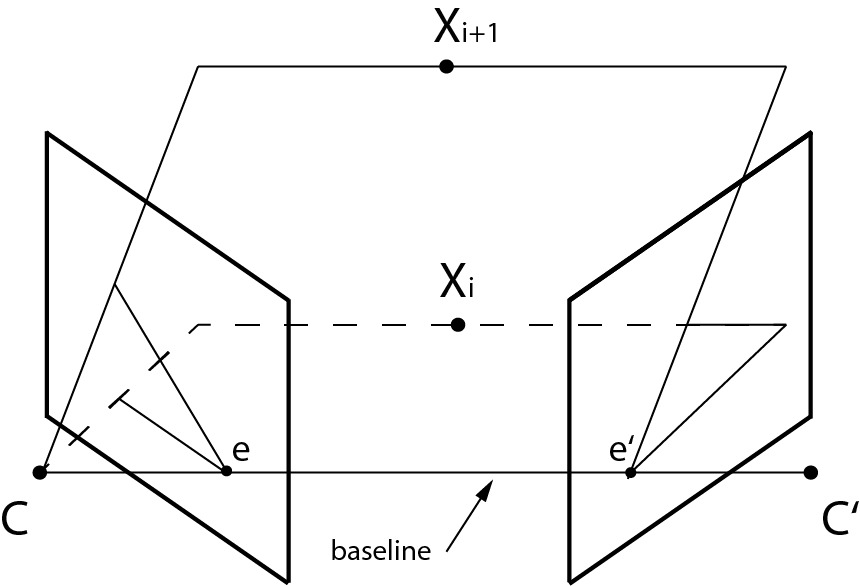
\includegraphics[width=0.7\textwidth]{figures/EpipolarGeometry_Planes}
		\caption[Pencil of epipolar planes with varying world points X]{Pencil of epipolar planes with varying world points $\mathbf{X}$ (\textit{source: own illustration based on} \cite[p.240]{Hartley.2011}).}
		\label{fig:EpiPlanes}
\end{figure} 

\subsection{Fundamental and Essential Matrix}
\index{Essential matrix}\index{Fundamental matrix}
The concept explained above can be represented algebraically as well - with the so called \textit{fundamental matrix}. The fundamental matrix can be derived in many ways, for the following derivation the projective geometry (see \autoref{ssec:projCam} as well as the epipolar geometry is needed. 

\note{It is important to clarify in which direction the rotation is interpreted, namely which camera view gets multiplied first or which coordinate system is used as a basis. The results are equivalent but differ in their appearance. In common literature there is no standardized order which makes it slightly difficult to compare different results with each other. One has to choose an order and should stick with it. All values are then only to be interpreted relatively to the chosen order of camera pairs.}

As mentioned above, each camera has its own projection matrix. Using parts of \autoref{eq:pinholeMapping} the two projection matrices can be defined as (\cite[p.309]{Luhmann.2014}):
\begin{equation}
 P=KR[I | 0]
\qquad
 P'=K'R'[I | -b]
\end{equation}

with the rotation matrices $R$ and $R'$, the calibration matrices $K$ and $K'$ and the base vector $b$. As already stated above, the corresponding image point $\mathbf{x'}$ lies on the epipolar line $l$. The map $\mathbf{x}\mapsto l'$ can then be defined by the fundamental matrix $F$. The fundamental matrix $F$ is a  homogeneous $3\times 3$ matrix which can be described with 8 degrees of freedom. It stores the relative orientation data, such as the interior orientation. It satisfies the following equation (taken from \cite[p.245 et seq.]{Hartley.2011}, \cite[p.2]{Loop.2001} and \cite[p.310]{Luhmann.2014})\footnote{Note: \cite{Luhmann.2014} actually defines it the other way around: $\mathbf{x}^T F \mathbf{x'} =0$. For the sake of clarity, the following euqations are all based on the order presented by \cite{Hartley.2011}. To achieve the respectively other  result one has to \textit{transpose} the fundamental matrix, which changes the order of the camera pair.}: 

\begin{equation}
 \mathbf{x'}^T F \mathbf{x}=0
 \qquad
\text{for any pair of corresponding points } \mathbf{x}\leftrightarrow \mathbf{x'}\label{eq:CoplanarityCondition} 
\end{equation}
 
This equation is also called the \textit{coplanarity condition}\index{Coplanarity condition} since it derives from the fact that the rays are coplanar.

For the \textit{epipolar lines}\index{Epipolar line} the following equations can be used (\cite[p.246]{Hartley.2011}):
\begin{equation}
 l' = F\mathbf{x}
 \qquad
\text{epipolar line corresponding to } \mathbf{x}\label{eq:epiLineL2}
\end{equation}
\begin{equation}
 l = F^T\mathbf{x'}
 \qquad
\text{epipolar line corresponding to } \mathbf{x'}\label{eq:epiLineL}
\end{equation}

Since all epipolar lines intersect at the \textit{epipoles}\index{Epipole}, these two points can be derived from \autoref{eq:epiLineL} and \autoref{eq:epiLineL2} respectively:

\note{To sum it up, the fundamental matrix $F$ describes the relationship between the camera $P$ and a second camera $P'$ - whichever cameras are associated as the first and the second camera is up to the programmer. $F^T$ then describes the opposite order $P',P$ (\cite[p.245]{Hartley.2011}.}
%%%%%%%%%%%%%%%%%%%%%%%%%%%%%%%%%%%%%%%%%%%%%%%%%%%% todos
\todo{absolute orientation --> p.310 Luhmann}
\todo{epipolar and essential matrix}\\
\todo{how many points are needed fundamental vs. essential --> p.310 luhman}\\
\enquote{In der Theorie benötigt der 8-Punkt-Algorithmus mindestens acht korrespondierende Punkte für die Berechnung der Fundamental-Matrix. Allerdings wird dabei eine hohe Genauigkeit der Werte vorausgesetzt. Bei einer manuellen Bestimmung der Punkte, hat es sich als sinnvoll herausgestellt, mehr als acht Korrespondezen zu wählen.}
%%%%%%%%%%%%%%%%%%%%%%%%%%%%%%%%%%%%%%%%%%%%%%%%%%%% /todos

With this computed geometry the relative pose and calibration for a pair of cameras in world space is known. The epipolar lines corresponding to a pixel in one image can now be used to find the corresponding pixel in the second view. For this, different corresponding algorithms can be used, such as \textit{optical flow}. Due to the computed epipolar geometry, the corresponding points only need to be searched along the epipolar lines. To speed up the search, the image pairs can be \textit{rectified} first (\cite[p.472 et seq.]{Szeliski.2011}).

\subsection{Image Rectification and Disparity}\label{ssec:RectificationDisp}
By \textit{rectifying}\index{Rectification} image pairs corresponding horizontal lines become epipolar lines, which means that all corresponding image points are then lying on the same horizontal lines. This makes the search for corresponding points much easier since the pixels do not have to be compared on \textit{skew lines} but can be compared only on the same \textit{scan lines} (\cite[p.1]{Loop.2001}).

\note{Although image rectification works the best for cameras which are standing next to each other, it can still be achieved in other scenarios as well. However, the input images should not be too verged and can not have too big of a size difference. Rectification is not a must and there are other methods to make the search for corresponding points easier, e.g. \textit{plane sweep}\index{Plane sweep}. In general, rectifying an arbitrary collection of images with non-collinear optical centers simultaneously is not possible (\cite[p.472 et seq.]{Szeliski.2011}).}

In rectification the pixel coordinates of the image pairs get transformed into other pixel coordinates with the help of 2-D projective transformations (\textit{homographies}). This is usually achieved by first rotating both cameras so that their viewing directions are perpendicular to their \textit{baseline}. Then, the cameras' \textit{up vectors} have to be made perpendicular to the camera center line. If the focal lengths are different, the images then need to re-scaled, magnifying smaller images. \autoref{fig:Rectify} illustrates possible rectification steps (\cite[p.1]{Loop.2001}, \cite[p.473]{Szeliski.2011} and \cite[p.436]{Luhmann.2014}).

Since the process of rectification is a science in its own, the author would like to suggest \cite{Loop.2001} as further readings for full details of this procedure.

The \textit{standard rectified geometry} leads to the following \enquote{simple inverse relationship} between disparities\index{Disparity} $d$ and 3-D depth values\index{Depth value Z} $Z$ (\cite[p.473]{Szeliski.2011}:

\begin{equation}
 d = f \frac{B}{Z} \label{eq:disparity}
\end{equation}

with the \textit{focal length} $f$ (in pixels), baseline $B$ and 

\begin{equation}
 x'=x+d(x,y,) 
 \qquad
 \text{with }
 y'=y
\end{equation}
for the computation of corresponding pixel coordinates.

With this the so called \textit{disparity map}\index{Disparity map} $d(x,y)$ can be estimated. The term \textit{disparity} is here used to describe the difference in locations of corresponding points. The information of corresponding pixels at similar locations are stored in a \textit{disparity space image} (DSI)\index{Disparity space image DSI} $C(x,y,d)$ (\cite[p.473]{Szeliski.2011}).

\begin{figure}[htbp]
		\centering
		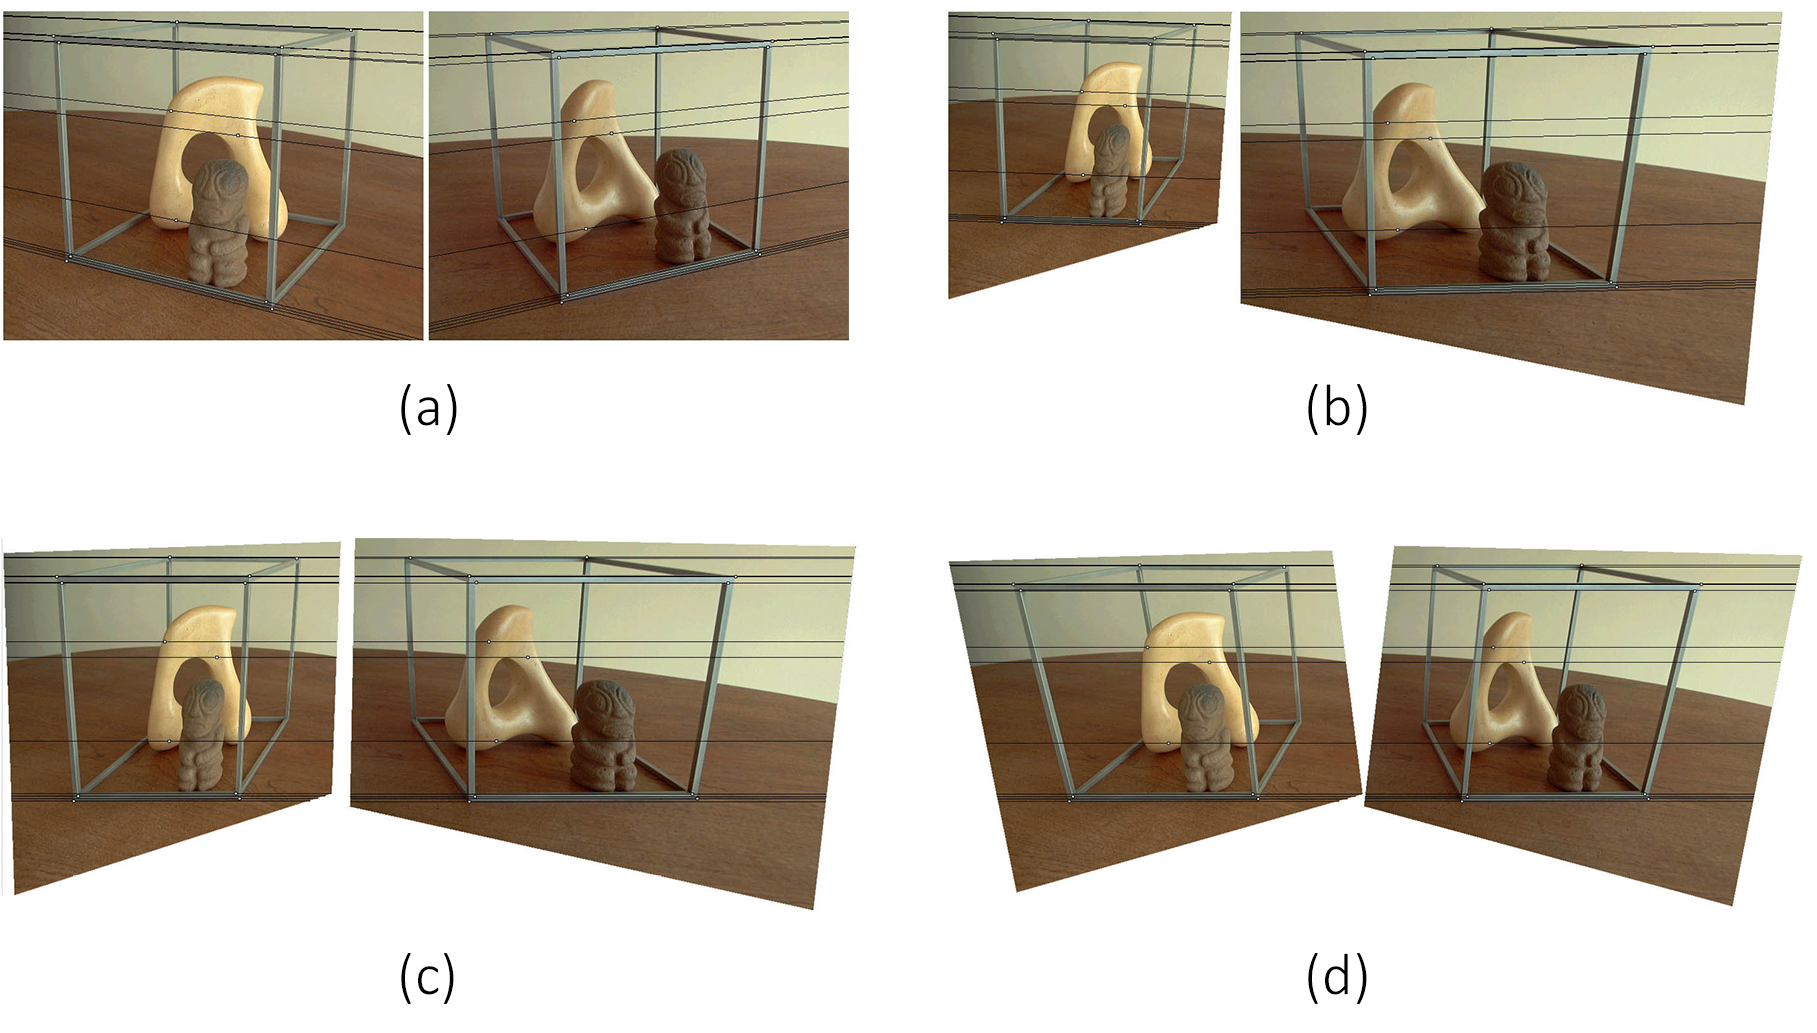
\includegraphics[width=1.0\textwidth]{figures/Rectify}
		\caption[Stages of the rectification algorithm]{Stages of the rectification algorithm proposed by \cite{Loop.2001}; \textbf{(a)} Original image pair with epipolar lines; \textbf{(b)} image transformation with projective mapping to make epipolar lines parallel to each other; \textbf{c} image transformation which rectifies the image pair - the epipolar lines are now horizontally aligned; \textbf{d} Final rectified image with reduced horizontal distortion    \textit{source:} \cite[p.12]{Loop.2001}).}
		\label{fig:Rectify}
\end{figure} 

%%%%%%%%%%%%%%%%%%%%%%%%%%%%%%%%%%%%%%%%%%%%%%%%%%%%%%% todos???
\section{What else?}
-introduction to stereo correspondence (see \cite[p.468]{Szeliski.2011})\\
-(surface) reconstruction? --> next steps\\
\todo{go to \cite[p.257 and 314]{Luhmann.2014} for a diagram!!!!}\\
\todo{describe stereo matching vs. structure from motion}\\
\todo{Triangulation?}

\begin{itemize}
\item use Markus Mann - StereoCameraCalibration.pdf !!!!
\item and Camera Calibration for Stereo Vision.pdf
\item Levenberg-Marquardt algorithm? \url{http://www.cs.ubc.ca/~lowe/papers/danm96.pdf}
\item RANSAC?
\end{itemize}
%%%%%%%%%%%%%%%%%%%%%%%%%%%%%%%%%%%%%%%%%%%%%%%%%%%%%%% /todos
